\subsection{State of the Art}
Indenfor skemalægning findes allerede nogle løsninger på de udfordringer, som nemt opstår indenfor skemalægning. Et af disse er USA Schedulers program kaldet School Master Scheduling Software\cite{USAS}, et program som først og fremmest tager de studerende i betragtning. Programmet er i stand til at lave funktionelle skemaer ud fra de studerenes ønsker, analysere de mest optimale løsninger ud fra ønskerne, og ud fra dette, undgår konflikter så som 2 moduler, der ligger oveni hinanden så studerende, der deltager aktivt i begge, bliver nødt til at vælge den ene fra.

Et andet stykke software kaldet Mimosa Scheduling Software\cite{Mimosa}, fokuserer mere på de grundlæggende udfordringer så som overbooking og nemt at kunne ændre på skemaerne, hvis der skulle komme en uventet udfordring. Det er i stand til at lave skemaer for lærere, elever, klasser og lokaler, alt det som enhver dansk folkeskole har brug for. Institutionerne henter programmet, laver deres egne ressourcer, hvilket vil sige lærere, elever, lokaler osv. og derefter fordeler de forskellige ressourcer ud over dagene. Programmet vil så fortælle om dette kan lade sig gøre, og hvis dette ikke er tilfældet, vil det fortælle hvorfor\cite{MimosaTutorial}. I modsætning til School Master Scheduling, er Mimosas program mere henvendt til skemalæggerne, og ikke så meget til de studerende. 

Begge programmer løser dog ikke selve skemalægningsprocessen, da dette stadig gøres manuelt af skemalæggeren, eller de individuelle studerende for deres eget skema, og ser man over top 10 mest anbefalede skemalægningsprogrammer\cite{top10Schedulers}, er de ikke rangeret ud fra automatisk skemalægning. Det, som kommer tættest på, vil være Auto-Scheduler, men denne funktionalitet virker kun for medarbejdere ud fra en historik, og er derfor ikke automatisk skemalægning. Besøger man et af de programmers hjemmesider, som er med i denne top ti anmeldelse, får man heller ingen information om de er i stand til netop dette. Et program, som vil være i stand til helt automatisk at lave skemaer til alle på for eksempel en dansk folkeskole, kun ud fra de ansatte, eleverne og klasselokalerne som er til rådighed, vil derfor være innovativt. Disse top-ti skemalægningsværktøjer er også mest henvendt til firmaer, så firmaerne kan tildele hver lønmodtager jobs og holde styr på, hvor meget løn hver lønmodtager får, hvilket er noget anmeldelsesiden går meget op i, og bedømmer hver skemalægningsværktøj ud fra.

På Tingstrup skole skal et program ved navn Tabulex tages i brug i forbindelse med skemalægningen. Det er et skemalægningsværktøj som de forrige. Programmet, ligesom de andre, kræver at brugeren stiller programmet en helt del krav, heriblandt hvordan lærerens tid skal prioriteres, hvornår lektionerne ligges, og hvor meget hver af disse regler skal prioriteres og overholdes af programmet\cite{Tabulex}. Tabulex kan selv forsøge i bedste fald, at lægge et skema ud fra de rigtigt mange begrænsninger, som skemalæggeren har stillet det, og undervejs vil programmet så lade personen som bruger programmet, vide hvis kravene som er opstillet, ikke kan lade sig gøre, og så brugeren kan rette dem til. Herefter er det så muligt at fortsætte lægningen, eller starte lægningen forfra. Ligesom de andre skemalægningsværktøjer, kommer det med en grafisk brugerflade, som understøtter drag\&drop, og som er rimelig overskuelig. Tabulex kan dog ikke holde styr på regnskabet ligesom værktøjerne i forhenværende afsnit, men dette er heller ikke hvad programmet er lavet til at håndtere. Udover dette, har Tabulex en fin dokumentation omkring hvordan programmet eksporterer til en .csv fil\cite{Tabulex_csv}, og da et af kravene stillet af vores case er at kunne inddrage skemaet i Skoleintra, KMD Elev og andet\cite{Interview_Kaerby}, er dette noget vi vil kigge nærmere på, eftersom disse andre programmer de benytter, tager imod .csv formaet.
\begin{figure}[h!]
	\centering
	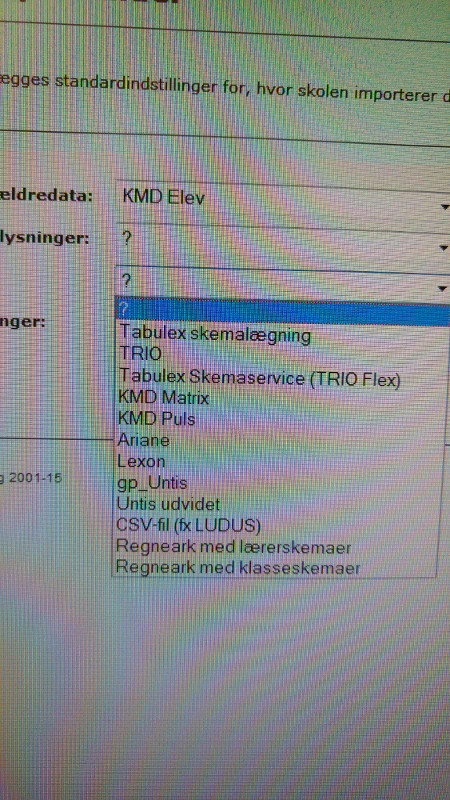
\includegraphics[width=0.4\textwidth]{../Billeder/Skemaimportering_filtyper_Intra.jpg}{}
	\label{fig:kompatibleFiltyper}
\end{figure}
\FloatBarrier
Et andet program skolen brugte, er KMD Educa, hvilket er en samling af forskellige værktøjer\cite{KMD} der gør det muligt blandt andet at vikarføre, lægge skemaer og håndtere karakterresultater for hver enkelte elev, som går på skolen og som har gået på skolen. Dette er en af de mange grunde, at Aalborg Kommune har valgt at benytte sig af KMD Educa programmet ``Elev''\cite{useCase_KMD_Educa_Elev}.

Vores case [Kærbyskolen] brugte et program kaldet Docendo før skolestart 2015, men selvom de selv siger at deres program er meget fleksibelt\cite{Docendo}, var det ikke fleksibelt nok for skolen, og de valgte derfor at ligge skemaet manuelt. Programmet tillader at lægge skemaet elektronisk, lave varierende lektionslængde og tælle brugte timer, så eleverne hverken får for lidt lektioner, eller alt for mange. Ud fra deres video\cite{Docendo_video}, er det nemt at gå til, klasserne kan holdes styr på i en grafisk brugerflade, lektionerne kan flyttes rundt som det passer en, og hvis man gør dette, adapterer tidspunktet i lektionsrubrikken også. Skemaet lægges dog for hver uge, men dette er i sidste ende ligegyldigt, da det tidligere uges skema godt kan genbruges.
